

\chapter{Elektronik}
\label{chap:elektronik}

\section{Das Gehirn des Bootes}
Für die Steuerung des Bootes wird ein Raspberry Pi Zero W 1.1 verwendet. Dieser verfügt über ausreichend Rechenenleistung um alle notwendigen Berechnungen in Echtzeit durchzuführen. Er verfügt über einen einkernigen ARM Prozessor, der mit 400 MHz getacktet ist. Sein Arbeitsspeicher beträgt 512 Megabyte. Er ist nur 6,5 mal 3,2 cm gross und wiegt nur 9 Gramm.

Auf dem Rasperry Pi läuft ein Debian basiertes GNU/Linux Betriebssystem. Im Kapitel Autonomie wird auf die Software detailliert eingegangen. 

Der Raspberry Pi Zero W 1.1 kann über WLan nach den Spezfikationen 802.11 b/g/n sowie über Bluetooth 4.1 und Bluetooth Low Energy (BLE) kommunizieren. Die  Wlan Verbindung wird benutzt, um mit dem autonomen Segelboot zu kommunizieren. Über die Verbindung kann der Rechner drahtlos aufgesetzt und eingerichtet werden. Auch die Übermittlung von Zielkoordinaten erfolgt über diese Verbindung. Die Bluetooth Verbindung wird nicht benutzt.
\begin{figure}[H]
    \centering
    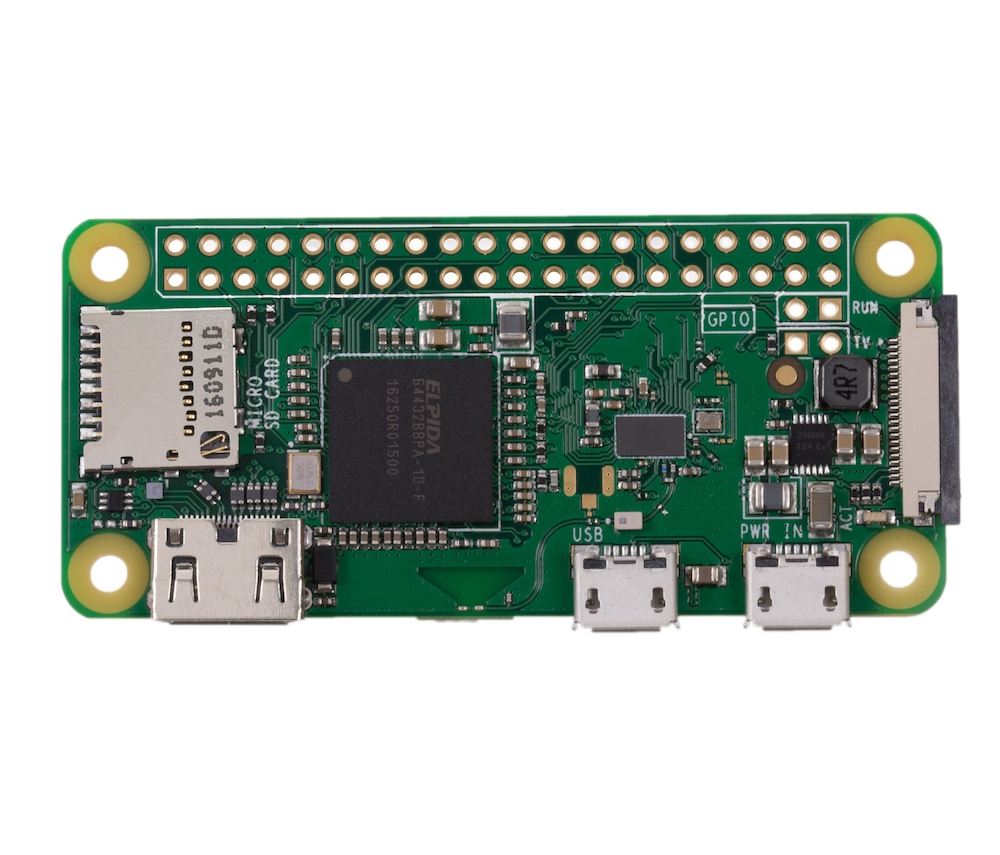
\includegraphics[width=0.5\linewidth]{assets/raspi Zero.jpg}
    \caption{Raspberry Pi Zero W}
    \label{fig:enter-label}
\end{figure}



Die in den unmittelbar nachfolgenden Abschnitten beschriebenen Sensoren und Aktuatoren sowie die Energieversorgung werden über die 40 GPIO (general-purpose input/output) Pins angeschlossen. 

Der Raspberry Pi Zero W 1.1 wird mit 5 V Gleichspannung betrieben. Sein Stromverbrauch ist sehr bescheiden. Seine maximale Spromaufnahme liegt bei 1,2 A [https://de.wikipedia.org/wiki/Raspberry_Pi#Eigenschaften]; im Leerlauf braucht er aber nur 120 mA.
[https://www.bitblokes.de/stromverbrauch-des-raspberry-pi-zero-w-mit-wlan-und-bluetooth-gemessen/ ]
\section{Sensoren und Aktuatoren}
\subsection{Positionsestimmung (GPS)}

Zur Positionsbestimmung also der Bestimmung des aktuellen Standorts des Segelboots, werden Funksignale des bekannten US-amerikanischen satellitenbasierten Global Positioning Systems (GPS) (deutsch Globales Positionsbestimmungssystem), offiziell NAVSTAR GPS verwendet. Dafür wird das Empfängermodul Whadda Neo 7M der belgischen Velleman Group nv verwendet, welches alternativ Signale des entsprechendenen russischen Systems GLONASS empfangen kann. 
\begin{figure}[H] 
    \centering
    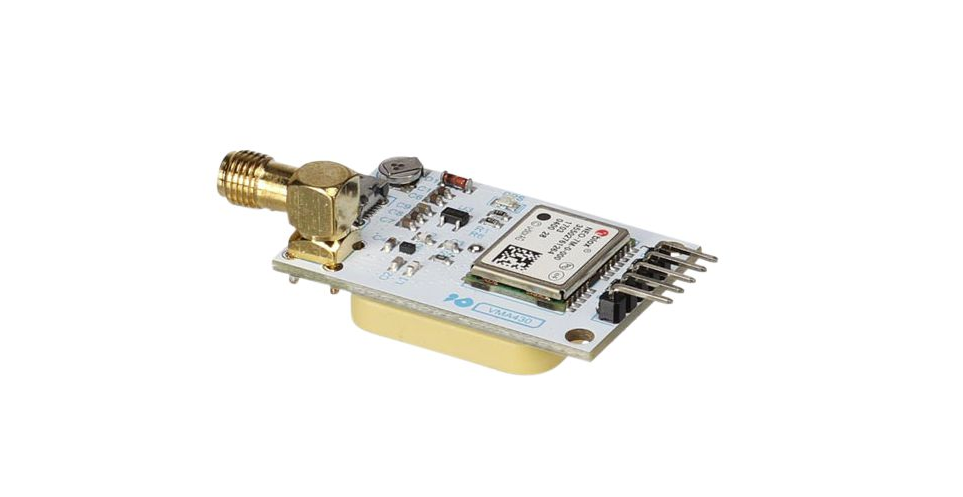
\includegraphics[width=1\linewidth]{gps.png}
    \caption{GPS Modul}
    \label{fig:gps}
\end{figure}
Das Modul verfügt über eine MicroUSB Schnittstelle. Diese wird aber nicht verwendet, weil der Raspberry Pi Zero W 1.1 nur über zwei MicroUSB verfügt, Kabel mit zwei männlichen MicroUSB Steckern aber nicht existieren und in den USB Spezifikationen nicht vorgesehen sind. 

Das Modul wird über die eben falls vorhandenen Pins mit dem Raspberry Pi Zero W 1.1 verdrahtet und  kommuniziert über eine serielle Verbindung. Die Pins 2 (TX) und 3 (RX) werden dabei mit den Pins 10 und 8 des Raspberry Pi Zero W 1.1 verbunden. Das Modul wird mit 5 V betrieben. Dazu wird sein Pins 5 (VCC) mit der 5 V Gleichspannungsleitung und sein Pin 4 (GND) mit der Ground Leitung der Stromversorgung verbunden.   
\begin{figure}[H]
    \centering
    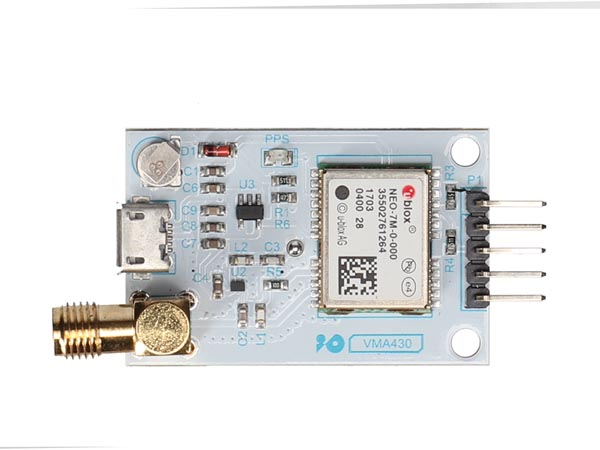
\includegraphics[width=0.75\linewidth]{vma430_front-1.jpg}
    \caption{GPS Modul - Oberseite}
    \label{fig:enter-label}
\end{figure}
Das Modul wird unter Deck im Rumpf des Bootes platziert. Weil für die Deckplatte eine dünne Sperrholzplatte verwendet wird kann auf eine externen Empfangsantenne verzichtet werden. Die vorhandene SMA Antennen Steckbuchse bleibt damit unbenutzt. Es wird die eingebaute keramische Patchantenne verwendet. In der unmittelbar untenstehenden Abbildung ist diese als rosa Fläche mit einbem metallenen Knopf auf einem beigen Körper sichtbar. Solche Antennen 
\begin{figure}[H]
    \centering
    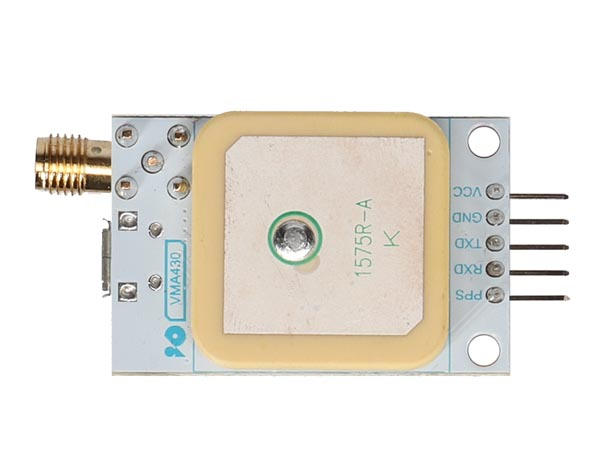
\includegraphics[width=0.75\linewidth]{vma430_back-1.jpg}
    \caption{GPS Modul - Unterseite}
    \label{fig:enter-label}
\end{figure}

\subsection{Gyro und Magnetometer}

Zur Bestimmung der Richtung des Segelboots dient ein Magnetormeter. Ein Magnetometer ist eine sensorische Einrichtung zur Messung magnetischer Flussdichten [https://de.wikipedia.org/wiki/Magnetometer]. Im voriegenden Projekt wird das Magnetormeter dafür eingesetzt, um damit einen Magnetkompass zu realisieren, indem das erdmagnetische Feld dreidimensional erfasst wird, um daraus die Bootsrichtung abzuleiten. Dieses Verfahren wird auch in Smartphones zur Richtungsbestimmung angewendet.  

Im vorliegenden Projekt wird dafür das Sensormodul Purecrea GY-273 QMC5883L der deutschen Purecrea GmbH vorgesehen. Das Modul ist zusätzlich mit einem Gyroskop (deusch: Kreiselinstrument) ausgestattet. Auch damit kann die Bewegung des Segelboots erfasst werden. Ausserdem erlaubt es die Bestimmung der   Schräglage des Segelbootes. Im vorliegenden Projekt wird dieser Wert aber nicht erfasst und ausgewertet.

\begin{figure}[H]
    \centering
    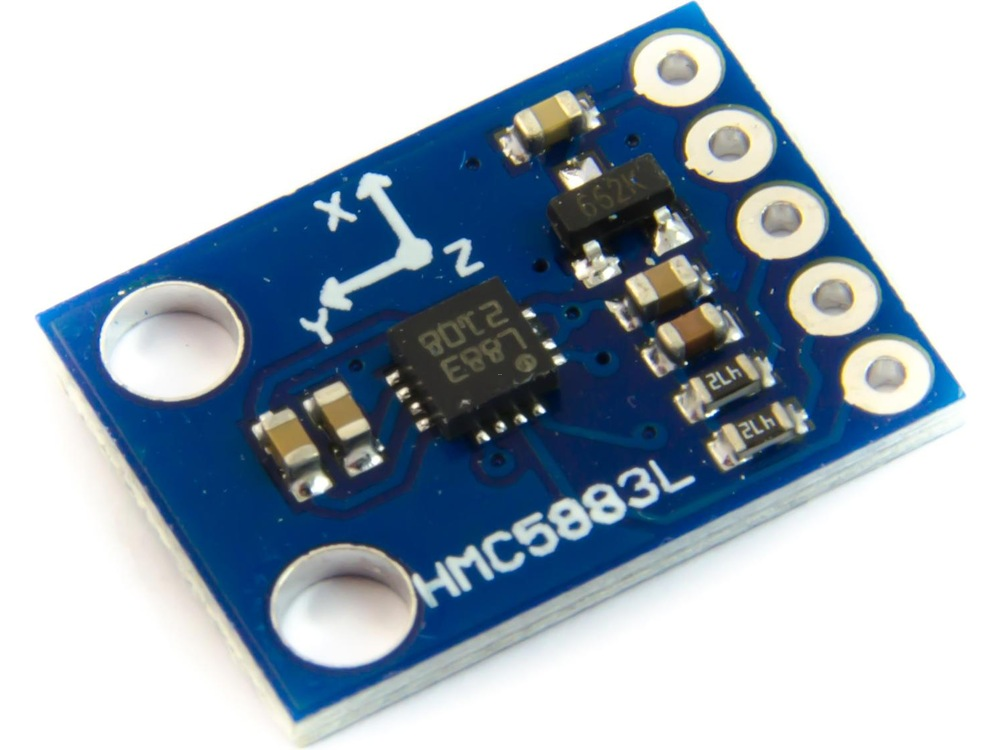
\includegraphics[width=0.5\linewidth]{assets/magnetometer.jpg}
    \caption{Gyro und Magnetometer}
\end{figure}

Das Sensormodul wird mit einer Eingangsspannung von 3-5 V Gleichspannung betrieben. Sein Pins 1 (GND) wird dafür mit der Ground Leitung und sein Pin 2 (VCC) wird mit der der 5 V Gleichspannungsleitung der
Stromversorgung verbunden.

Die Kommunikation mit dem Raspberry Pi Zero W 1.1 erfolgt über eine serielle Verbindung. Der Pin 4 (SCL) und der Pin 5 (SDA) des Moduls werden dafür mit den Pins 5 und 19 des Raspberry Pi Zero W 1.1 verdrahtet.

\subsection{Eigenentwicklung des Windrichtungssensor}
Der Windrichtungssenor muss selbst entwickelt und gebaut werden, da die am Markt angebotenen  Windrichtungsmesser entweder zu gross und zu schwer sind, Energiemengen benötigen, die auf dem autonomen Segelboot nicht zur Verfügung stehen oder unerschwinglich teuer sind.

Windrichtungssensoren lassen sich in zwei unterschiedliche Typen einteilen. Der erste Typ verwendet ein Pontiometer zur Richtungsbestimmung. Solche Messgeräte sind mechanisch sehr leicht umzusetzen, da dazu lediglich ein kleiner Flügel an der Achse eines Potentiometers befestigt werden muss. Die Position des Flügels kann damit über einen analogen Input Pin mit einem Microcontroller eingelesen und daraus die Richtung des Windes abgeleitete werden. Der Nachteil dieses Typs ist, dass die freie Drehung der Achse durch die Reibung das Potentiometers stark abgebremnst wird. Dieser Typ wird daher nicht weiter verfolgt.

Der andere Type verwendet Hall Sensoren, welche den Hall-Effekt zur Messung von 
Magnetfeldern nutzen [https://de.wikipedia.org/wiki/Hall-Sensor]. Sie sind passive Sensoren, die den Spannungsunterschied messen, der an einem elektrischen Leiter erzeugt wird, wenn ein Magnetfeld senkrecht zur Fliessrichtung eines elektrischen Stroms steht [https://at.rs-online.com/web/content/discovery-portal/produktratgeber/hall-sensoren-leitfaden]. Um die Rotation eines Objektes mittels Hall Sensoren zu messen gibt es die folgenden zwei Möglichkeiten. 

Bei der ersten Variante wird um ein abwechselnd magnetisch positiv und magnetisch negativ geladenes rundes Objekt mehrere Hall Sensoren platziert. Damit kann dann die Drehung des Objektes gemessen werden. Diese Variante ist praktisch schwierig umzusetzen, weil viele Hall Sensoren präzis kreisförmig um eine Achse angeordnet werden müssen. Dafür müssten die Hall Sensoren in enger Folge auf einer individuell entworfenen Platine verlötet werden. Der Entwurf einer solchen Platine ist anspruchsvoll, mit deren Herstellung müssten Auftragsfertiger beauftragt werden, was hohe Kosten verursachen würde. Weil die Hall Sensoren sehr eng aneinander platziert werden müssten, müssten sogeannte SMD Varianten (Surface Mountable Device; deutsch: oberflächenmontierbare Bauteile) verwendet werden, die ohne Bohrungen direkt auf die Oberfläche der  Platine gelötet werden. Es braucht dafür eine spezielle Löttechnik und die Gefahr, dass Bauteile beim Lötvorgang den Hitzetod sterben ist erheblich, wenn der Lötende über wenig Übung verfügt. Diese Varianten wird daher nicht weiter verfolgt.

Die zweite Varianten ist praktisch einfacher umzusetzen. Statt normale Hall Sensoren werden dabei spezielle, sogenannten Rotary Hall (deutsch rotierende magnetische Hall) Encoder verwendet. Ein Encoder (oder Messwertgeber) dient in der Antriebstechnik zur Signalbildung aus mechanischen Bewegungen. Er erkennt die Position einer Antriebseinheit (Welle) und gibt diese als elektrisches Signal aus. [https://www.kc-co.com/de/glossar/encoder/]. Rotary Hall Encoder sind komplexe Bauteile die fast immer als System-on-Chip gefertigt, in dem integrierte Hall-Elemente, analoges Frontend  und digitale Signalverarbeitung in einem einzigen Gerät integriert sind. Zur Messung des Winkels wird nur ein einfacher zweipoliger Magnet benötigt, der sich der sich über oder unter der Mitte des Chips dreht.
Zur Funktiosweise von Rotary Hall Encodern: Josef Janisch, Understanding Integrated Hall Effect Rotary Encoders, Nov 1, 2006 1:00am, auf Fierce Electonics (www.fierceelectronics.com/components/understanding-integrated-hall-effect-rotary-encoders). 

Da der Für das vorliegende Projekt wird ein Windsensor auf der Basis eines Rotary Hall Encoders vorgezogen. Dabei wird der auf einem Adapterboad gelötete AS5040-ASST der österreichischen ams-OSRAM AG verwendet. Das ist ein berührungsloser Rotary Hall Encoder für genaue Winkelmessung über eine volle Umdrehung von 360°.  Die absolute Winkelmessung liefert eine sofortige Anzeige der die Winkelposition des Magneten mit einer Auflösung von 0,35° = 1024 Positionen pro Umdrehung. Diese digitalen Daten sind als serieller Bitstrom und als PWM (Pulsweitenmodulation) Signal zur Verfügung. Für das vorliegende 
Darüber Projekt wird der serielle Bitstrom genutzt. 

Der Encoder kann mit 3,3V oder 5V betrieben werden. Quellen für beide Spannungen sind auf dem Segelboot vorhanden. Es wird der 3.3V Anschluss an Pin (.::::::::::::::::::::::......) des Raspberry Pi Zero W 1.1 genutzt.

\begin{figure}[H]
    \centering
    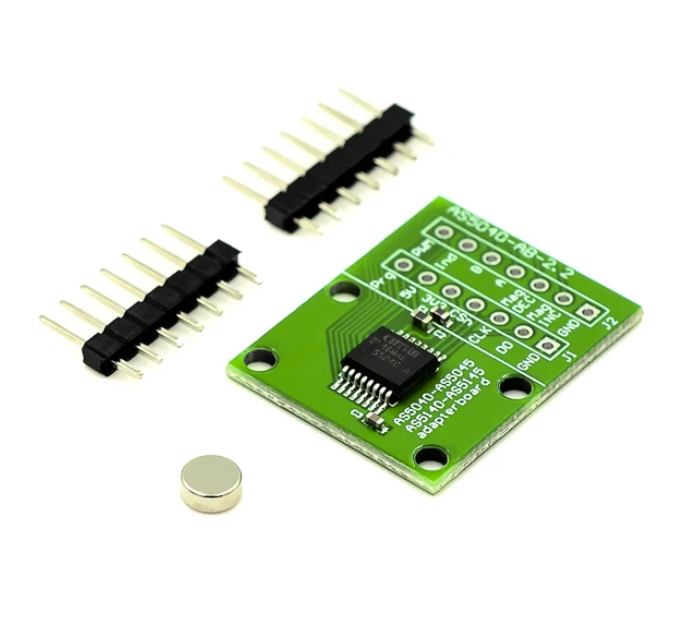
\includegraphics[width=0.5\linewidth]{assets/as5040image.png}
    \caption{AS5040-ASST mit Adapter Board}
    \label{fig:as5040}
\end{figure}

Verkablung

Bau de Windmessers aus gedruckten Teilen. 
Das Gehäuse des Windmesser besteht aus vier 3D gedruckten Teilen. Der obere Teil, der sich mit dem Wind dreht, ist so gebaut, dass er sich dank einem fahnenählichen Teil mit dem Wind dreht. Ebenso wird darauf geachtet, dass der Massemittelpunkt genau auf dem Drehpunkt liegt, damit die Messwerte auch dann genau sind, wenn das Boot nicht gerade ist. 

\begin{figure}[H]
    \centering
    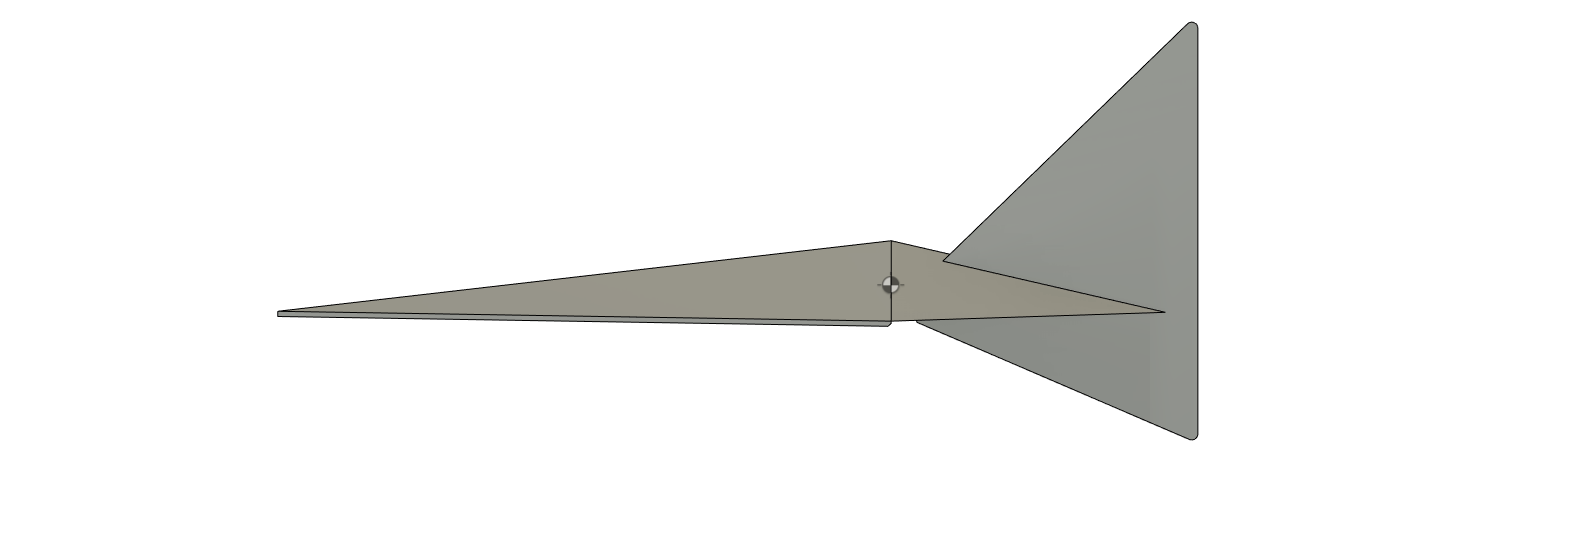
\includegraphics[width=0.75\linewidth]{assets/windsensor_top.png}
    \caption{Windsensor Top}
    
\end{figure}

Ebenso wurde ein Gehäuse für den Sensor gedruckt, bei welchem der Encoder und der Magnet immer richtig Ausgerichtet sind.
\begin{figure}[H]
    \centering
    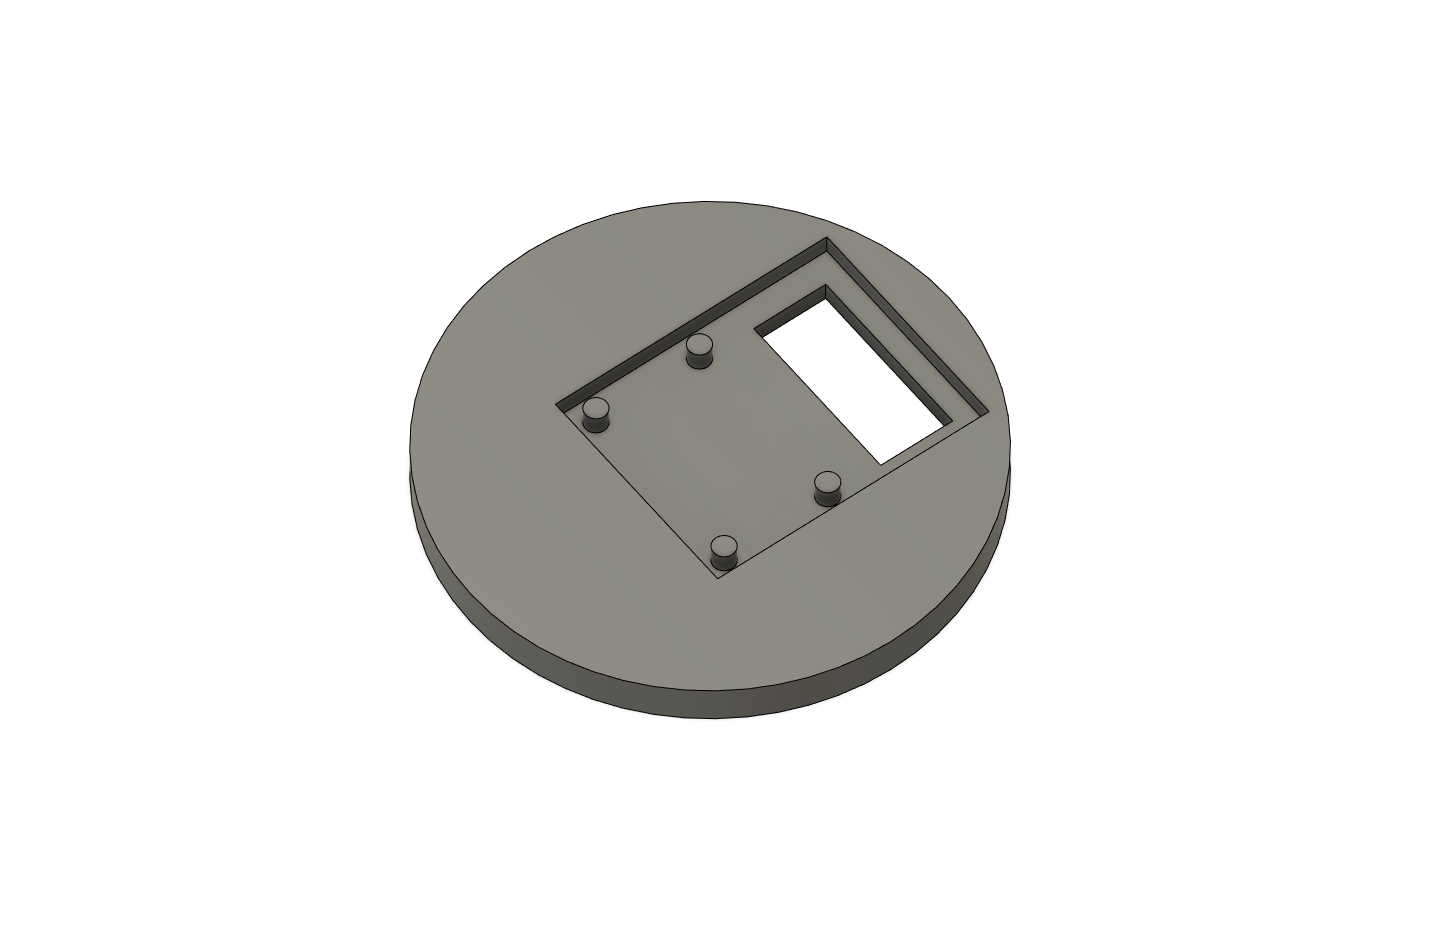
\includegraphics[width=0.5\linewidth]{assets/image.png}
    \caption{Bodenplatte um das Adapterplätchen richtig zu positionierten}
    
\end{figure}

\subsection{Aktuatoren}
Für die Bewegung des Ruders und des Sailflaps werden Aktuatorn verwendet. Aktuatoren (auch als Aktoren bezeichnet) sind das signalwandlerbezogene Gegenstück zu Sensoren. Sie setzen bei einem Bewegungsregelungsvorgang Signale durch mechanische Arbeit in Wirkungen um [https://de.wikipedia.org/wiki/Aktor]. Zur Bewegung von Ruder und Sailsflaps werden elektrische lineare Aktuatoren benötigt. Ein elektrischer Linearantrieb ist ein Gerät, das die Drehbewegung eines Wechsel- oder Gleichstrommotors in eine lineare Bewegung umwandelt. Er kann sowohl Schub- als auch Zugbewegungen ausführen.

Für das vorliegende Projekt werden zwei L16-100-63-6 Serie R Aktuator der kanadischen Actuonix Motion Devices Inc. verwendet. Diese sind für den Einsatz in der Robotik und im Modellbau entwickelt worden und wasserdicht. Damit sind  sie für den Einsatz  auf Segelbooten prädestiniert. 

Die Aktuatorachese kann um maximal 100mm ausgefahren werden. Die Maximalgeschindigkeit liegt ohne Last bei 20 mm/s. Damit sind sie nicht besonders schnell, verfügen mit 100N Stoss- und 46N Zugkraft aber über ausreichen Kraft zur Bewegung von Ruder und Sailflaps. Ihr Peak Power Point (der spezifische Geschwindigkeits- und Kraftpunkt, an dem die grösste Leistungsabgabe erfolgt), liegt bei 75N bei 10 mm/s. Das Getriebe der Akltuatoren weist eine Übersetzung von 63:1 auf. 

Die Aktuatoren verfügen über kein digitales Positionsfedback, dass heisst, dass nicht abgefragt werden kann, an welcher Position sich das Ende der ausfahrbahren Achse befindet. Es können jedoch konkrete Distanzen angesteuert werden. 

Die Aktuatoren weisen einen Normeingangsspannung von 6V auf, können aber auch mit der vorhandenen 5V Quelle betrieben werden, was aber zu einer leicht reduzierten Geschwindigkeit und Kraft führt. Für den Einsatz werden die Aktuatoren mit der  5 V Gleichspannungsleitung und der Ground Leitung der Enegerieversorung   verbunden. 

Über eine einzige Datenleitung  können kurze Impulse zwischen 1ms-2ms gesendet werden, wobei 1ms den Aktuator in die Startposition führt und der Aktuator bei 2ms voll ausgefahren wird. Um Einstellungen dazwischen zu erhalten, wird ein Wert zwischen 1ms und 2ms gesendet. 

\begin{figure}[H] 
    \centering
    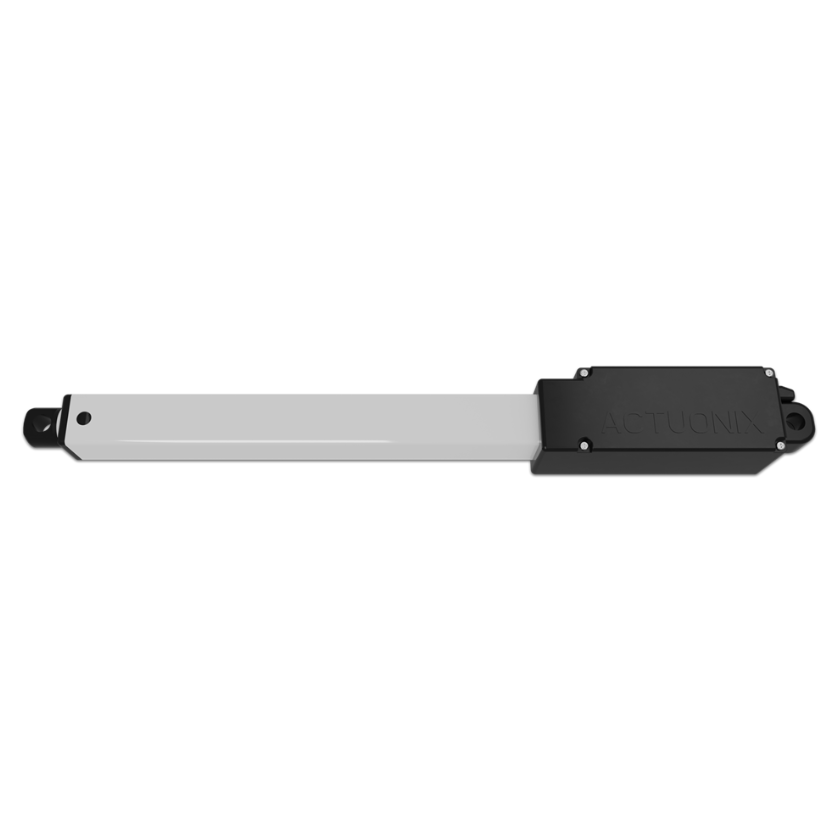
\includegraphics[width=0.5\linewidth]{actuonix.png}
    \caption{Actuonix Aktuator}
    \label{fig:actuator}
\end{figure}

\section{Schleifring (Slip Ring}


Text fehlt


\section{Energieversorgung}

Rechner, Sensoren und Aktuatoren werden mit elektrischer Energie betrieben. Weil das Segelboot vollkommen autonom funktionieren soll, muss diese auf dem Schiff selbst gewonnen werden. In Frage kommen dabei grundsätzlich drei Energiequellen, nämlich Wasserenergie, Windenergie und Sonnenenergie. 

\subsection{Wasserturbine}
Da sich das Boot im Wasser bewegt, könnte eine kleine Wasserturbine am Bootskörper befestigt und die Strömung zu deren Antrieb genutzt werden. Da sich das Boot relativ zum Wasser bewegt, gelten die gleichen Prinzipien wie bei Generierung elektrischer Energie durch Wasserkraft in Fliessgewässern.

Diese Methode hat jedoch gewichtige Nachteile. Segelboote erreichen, abgesehen von speziellen Konstruktionen wie sog. Foilingboote, bei denen der Bootskörper bei Fahrt vollständig aus dem Wasser gehoben wird, nur bescheidene Geschwindigkeiten. Da die Leistung einer Turbine in einer Flüssigkeit bei gleicher Fläche kubisch zur Strömungsgeschwindigkeit ansteigt, erlaubt diese Methode selbst bei idealen Segelbedingungen nur eine geringe Energieausbeute. Zudem würde das Segelboot durch die Turbine empfindlich abgebremst. 

\subsection{Windturbine}
Auch die Generierung von elektrischer Energie mithilfe einer Windturbine unter Nutzung der Windkraft ist nicht praktikabel. Um die Windenergie in Bewegungsenergie umzusetzen, aus der dann elektrische Energie generiert werden kann, muss ein Windrad in den Wind gedreht werden. Ein Segelboot kann keinen Kurs gegen den Wind segeln. Der Kurs vor dem Wind (also ein Kurs, bei dem der Wind von hinten auf das Boot trifft) ist zwar möglich, aber wenig effizient. Ein Windrad könnte folglich nicht fix mit dem Boot verbunden werden, sondern müsste drehbar ausgelegt werden, damit es unabhängig vom Kurs des Bootes in den Wind gedreht werden kann. Es müsste so platziert werden, dass nicht nur eine Berührung des Segels, sondern auch eine Berührung der Wasseroberfläche bei einer Kränkung (Schieflage) des Bootes ausgeschlossen ist. Damit müsste es am äussersten Bug, am äussersten Heck oder auf dem Mast platziert werden. Alle Positionen verbieten sich, da damit die Balance des Bootes akut gefährdet wäre. 

Schliesslich würde eine Positionierung am Bug oder Heck, je nach vorherrschendem Wind, zu einer vollen oder teilweisen Abschattung des Windrades durch das Segel oder des Segels durch das Windrad führen. Eine Positionierung auf dem Mast würde selbst im Fall eines Vertikalwindrades zu Verwirbelungen führen, welche die Segeleigenschaften des Bootes negativ beeinträchtigen würden. 

Einfluss auf den Kurs, da das Boot nicht verankert ist. Damit geht Energie verloren, da das Boot „weggeschoben“ wird, statt die Windenergie in nutzbare Drehung umzutzen.

\subsection{Photovoltaik}
Für die Nutzung der Sonnenenergie kommt nur die Methode der Photovoltaik in Frage. Die für den Betrieb von Wärme-Kraft-Maschinen erforderlichen Temperaturen lassen sich auf einem beweglichen Boot mit Sonnenenergie nicht erreichen.

Die Energieerzeugung mittels Photovoltaikanlagen ist auf Segelbooten bliebt und verbreitet. Solche Anlagen haben keinen Einfluss auf die Segeleigenschaften des Bootes. Die Energieausbeute hängt aber stark vom Sonnenstand und dem vorherrschenden Wetter ab. Im Gegensatz zu stationären Anlagen lassen sich Photovoltaikanlagen auf Booten nicht ideal auf die Sonne ausrichten und können je nach Kurs sogar vom Segel beschattet werden. Da während der Nachstunden überhaupt keine Energie gewonnen werden kann, muss das Boot zur Überbrückung zwingend mit einem Energiespeicher ausgerüstet werden.

\begin{itemize}
    \item Montage segel vs deck
    \item deck einfacher weil flach
    \item auswahl des Panels
    \item Grössenbeschränkung
    \item anforderungen an Laistungd es Panels
    \item Kompellt panel gekauft
    \item USB ausgang 5V
    \item Kostengünstig
    \item Outdoor einsatz Mobil entworfen worden das panel = Robust


\end{itemize}

\subsection{Enegiespeicher}
Während der Nachtstunden kann mit dem Solarpaneel keine Energie gewonnen werden kann und bei Nebel ist die Energieausbeute sehr gering. Daher muss das Boot zur Überbrückung dieser Phasen mit einem Energiespeicher ausgerüstet werden, damit seine Autonomie sichergestellt ist.

Es wurde vorgesehen, dass die Energiereserve einen Betrieb während drei Tagen (72 h) erlauben soll. Der genaue Energieverbrauch des Rechners, der Sensoren und vor allem der Aktuatoren hängt stark davon ab, wie oft Steuereingriffe vorgenommen werden müssen und Messdatenerfassungen, Neuberechnungen erfolgen. Es lässt sich daher nicht präzis berechnen, sondern nur abschätzen. 

Der Schätzwert für den Gesamtenergieverbrauch pro Stunde beträgt 1.5 Watt (bei 5 Volt Gleichspannung). Das ergibt einen Energieverbrauch von 36 Wattstunden pro Tag (24 h). Zur Überbrückung der vorgesehenen drei Tagen ohne Energiezufuhr muss der Speicher daher über eine Kapazität von mindestens 108 Wattstunden verfügen. 

Eine völlige Erschöpfung des Energiespeichers kann diesen schädigen, und muss daher verhindert werden. Aber bereits ein Absinken der Ladung auf unter 20 Prozent verkürzt dessen Lebensdauer. die Kapazität muss daher erhöht werden. Um über ausreichen Reserven zu verfügen, wird daher eine Kapazität von 185 Wattstunden vorgesehen.

Im Handel erhältliche sogenannte Powerbanks verfügen über eine Kapazität von bis zu 20'000 mAh, was eine Leistung von 100 Wh ergibt. Eine solche Powerbank genügt den gestellten Anforderungen damit nicht. Auch eine Kombination mehrerer Powerbanks scheidet aus, weil heute angebotene Geräte nicht auf die sogenannten Durchgangsladung (pass‐through charging) ausgelegt sind. Sie können also nicht geladen werden, während ein Verbraucher Energie bezieht.  

Deutlich grössere Powerstations, die insbesondere für den Campingeinsatz vorgesehen sind, verfügen über deutlich grössere Kapazitäten und sind duchgangsladungsfähig. Sie sind aber meist auf Verbraucher ausgelegt, die mit 220 V Wechselspannung betrieben werden,sind meist weit über 10 Kg schwer und kosten über 1000 Franken. Sie scheiden daher ebenfalls aus.   

Es muss daher auf eine Eigenentwicklung zurückgegriffen werden. Gängig dafür sind 18650 Li-ion Zellen. Die verwendeten Zellen verfügen über eine Akku Kapazität von 2'500 mAh bei 3.7 V. 
Der Akku wird in zwei Teile unterteilet, welche untereinander Parallel Geschalten sind. So bleibt die Spannung die selbe, jedoch erhöt sich die Kapazität. Die beiden Teile werden dann Seriel miteinander Vebunden. Somit ergibt sich eine Spannung von 7.4V und 25000mAh. 

Die einzelnen Zellen werden untereinander mit einem Nickelband verbunden, welches mit einem Punktschweissgerät direkt auf den Zellen verankert ist. Hierfür muss Spezialwerkzeug erworben werden, da ein solches Punktscheissgerät nicht zur Standartausrüstung einer Werkstatt gehört. Hier wird von den definierten Anforderungen abgewichen, da ein verlöten der Zellen technisch durchaus möglich wären, langes erhitzen durch den Lötkolben, könnten diese jedoch Permanent beschädigen und zu Feuer führen. Aus Sicherheitsgründen wird daher hier abgewichen. 




\begin{figure}[H]
    \centering
    \includegraphics[width=0.75\linewidth]{assets/akku_transparent.png}
    \caption{Selbstgebauter Akku}
    \label{fig:enter-label}
\end{figure}


\subsection{Ladeeletronik und Spannungswandelung}

Da Litiumzellen beim einer Überladung oder bei einer Entladung beschädigt oder im schlimmsten Fall in Flammen aufgehen, wird ein \ac{bms} (Battery Managment System) verwendet. Diese werden mit dem Plus und Minus Pol Verbunden. Zudem gibt es eine PM Verbindung, nach dem ersten Teil der seriellen Hälfte.


\begin{figure}
    \centering
    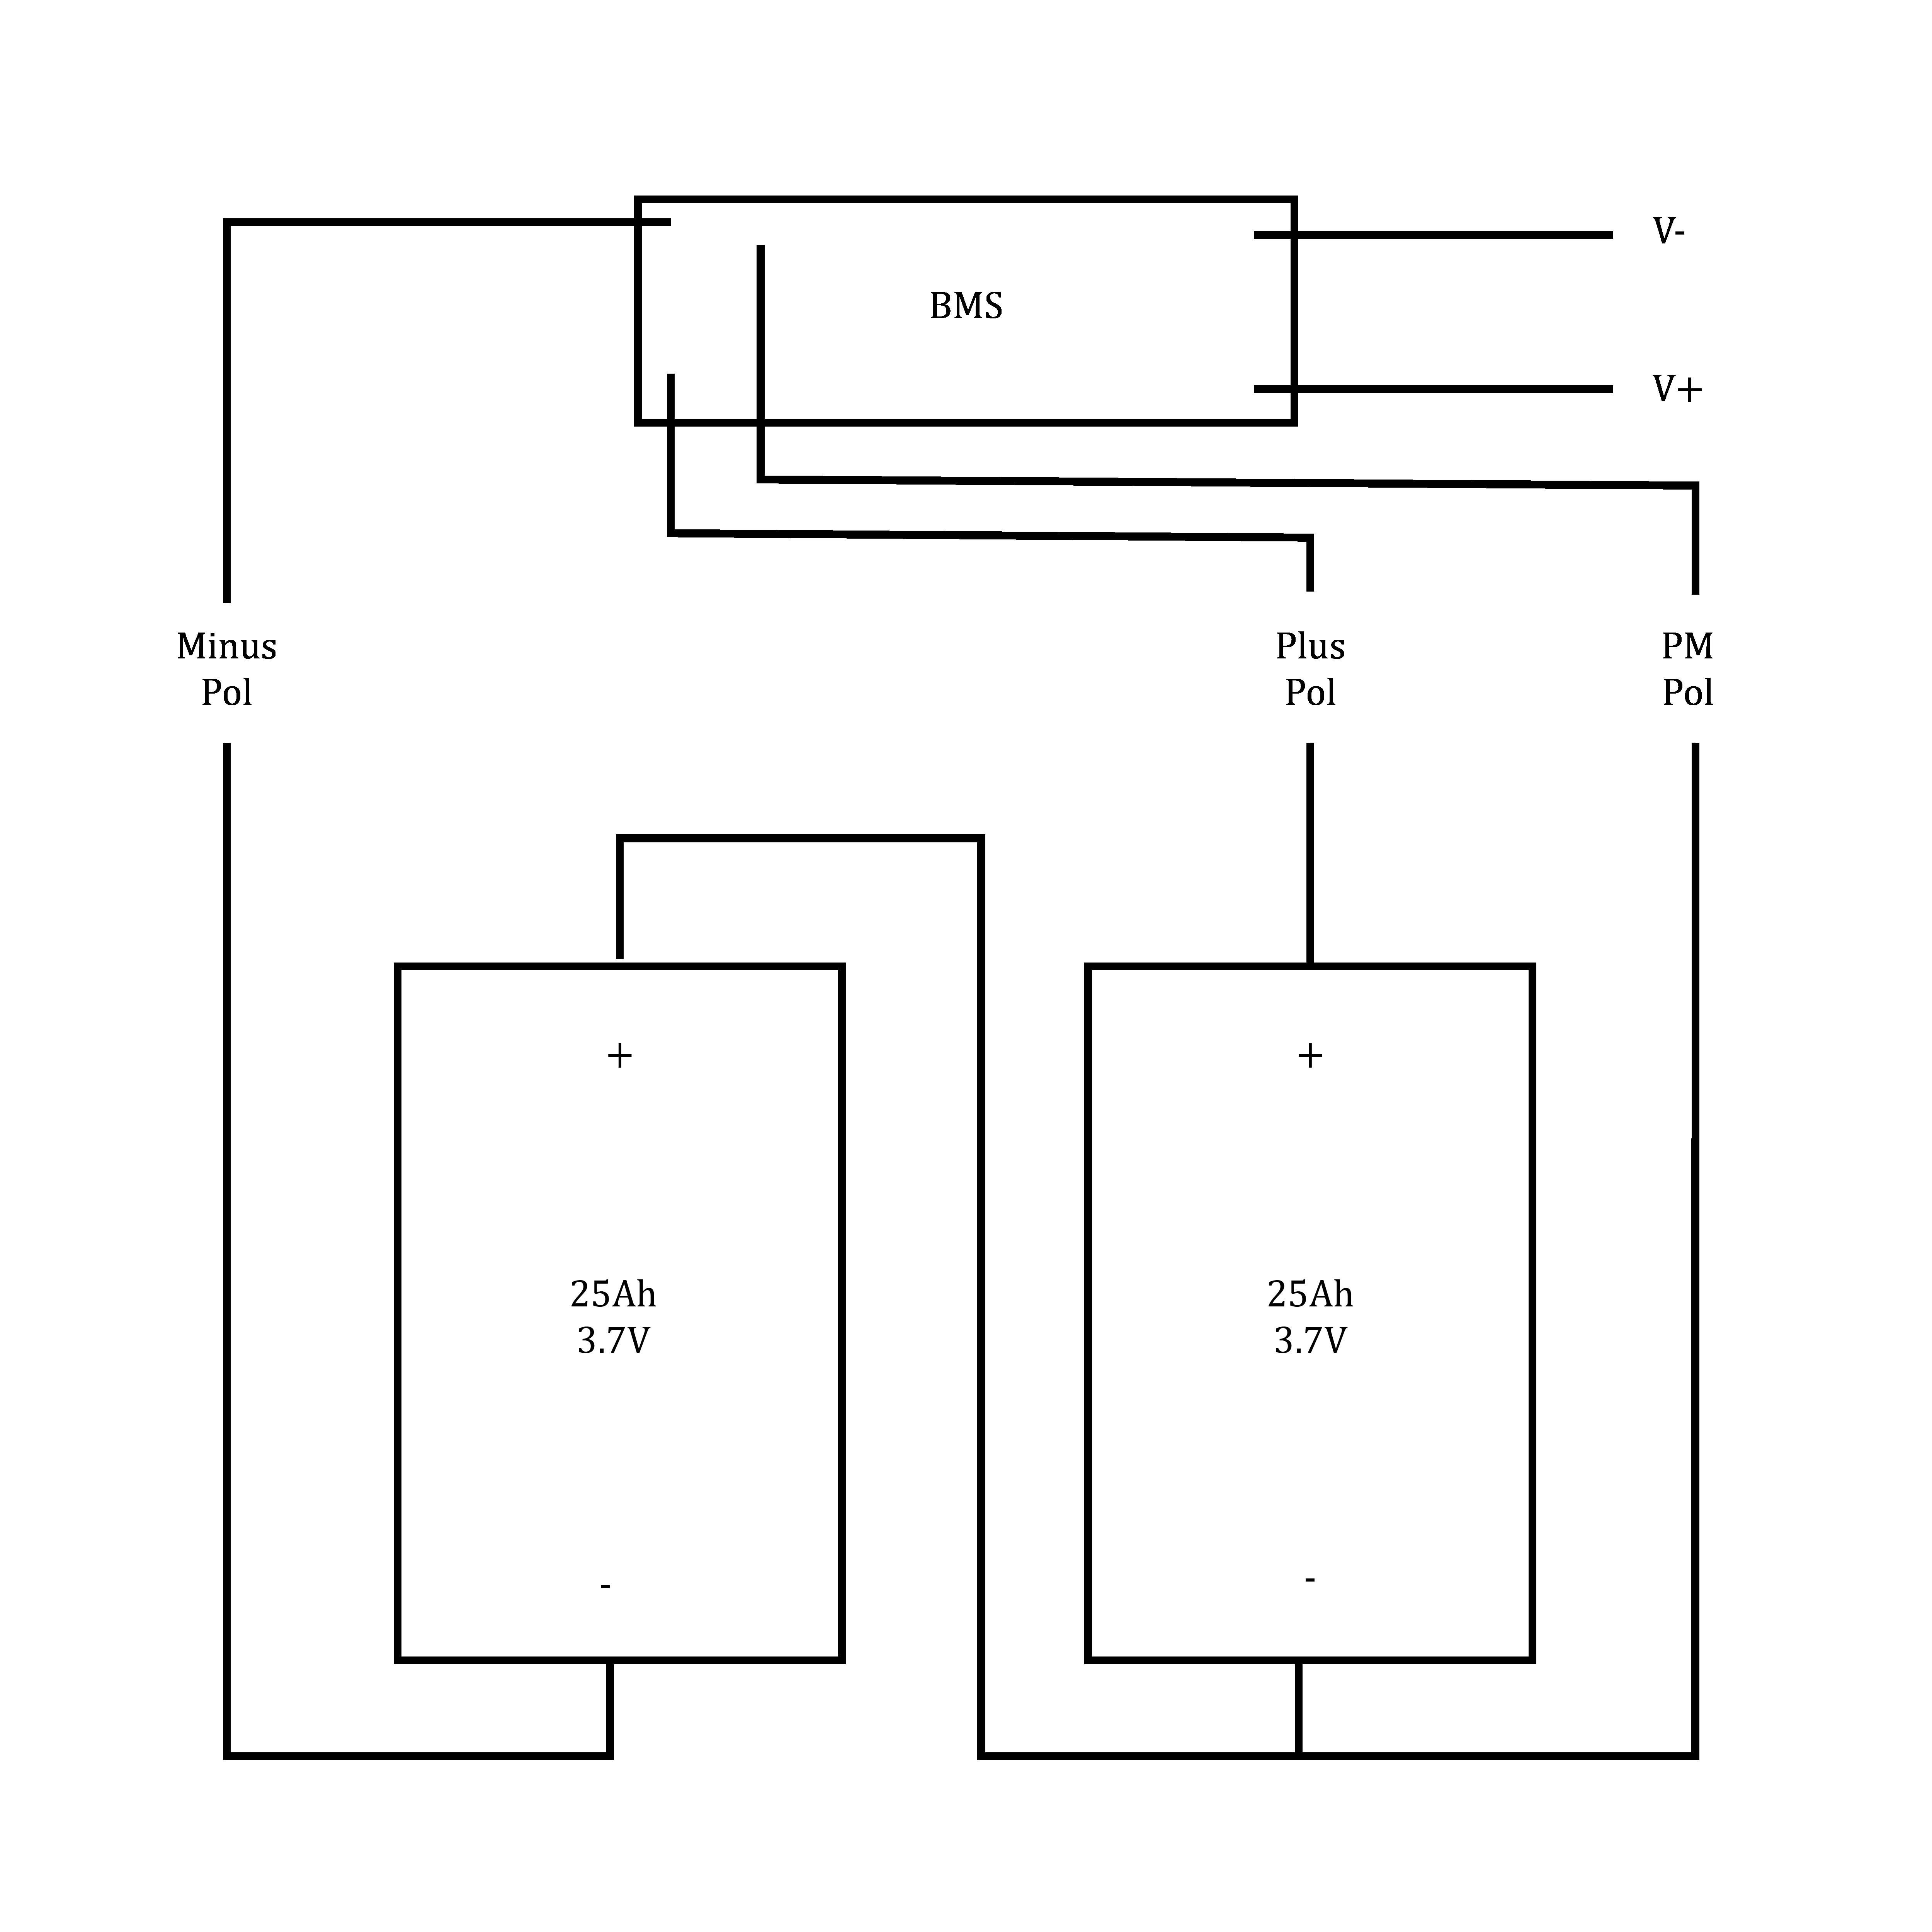
\includegraphics[width=0.75\linewidth]{assets/bms_circuit_image.png}
    \caption{BMS Circuit}
    \label{fig:enter-label}
\end{figure}
